%--------------------
\begin{figure}[h]
	\begin{center}
	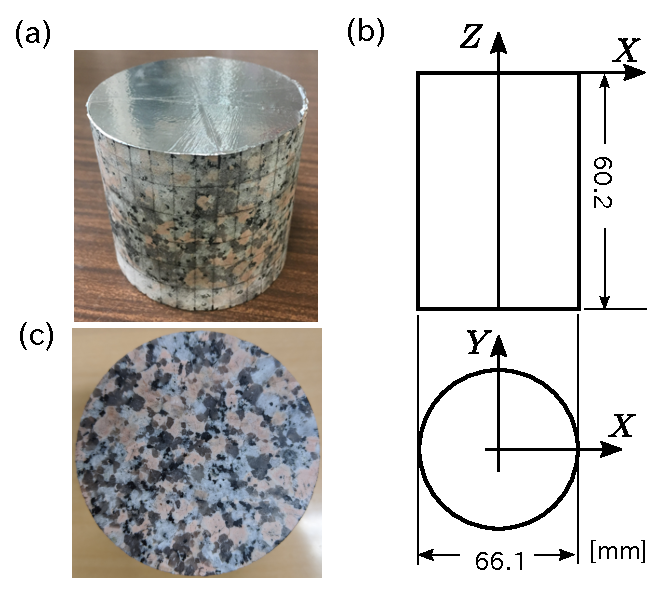
\includegraphics[width=0.6\linewidth]{Figs/fig1.eps} 
	\end{center}
	\caption{
		超音波計測に用いた花崗岩コア試料(万成花崗岩).
	} 
	\label{fig:fig1}
\end{figure}
%--------------------
%--------------------
\begin{figure}[h]
	\begin{center}
	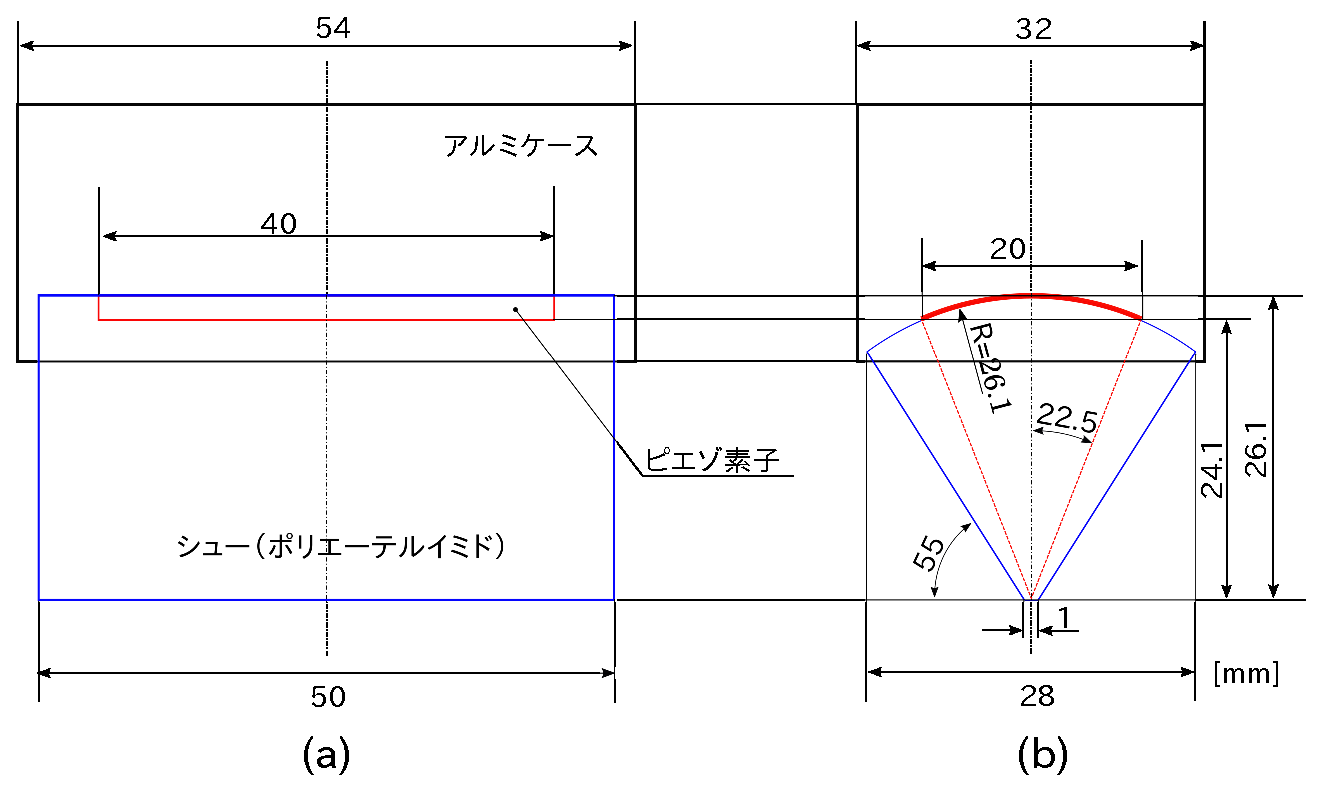
\includegraphics[width=0.8\linewidth]{Figs/fig2.eps} 
	\end{center}
	\caption{
		接触型ラインフォーカス探触子の形状と寸法.
	} 
	\label{fig:fig2}
\end{figure}
%--------------------
%--------------------
\begin{figure}[h]
	\begin{center}
	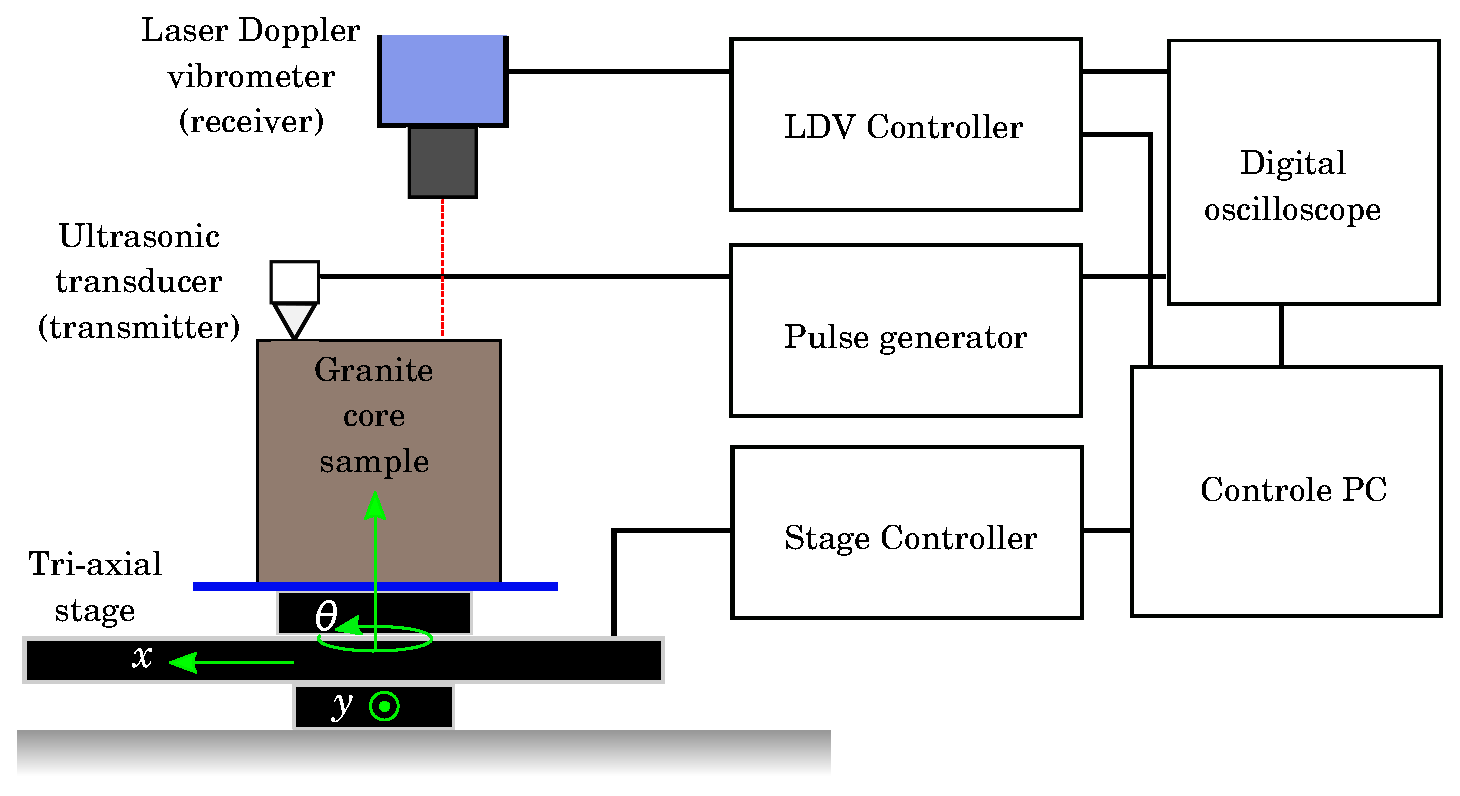
\includegraphics[width=0.8\linewidth]{Figs/fig3.eps} 
	\end{center}
	\caption{
		超音波測定装置の構成.
	} 
	\label{fig:fig3}
\end{figure}
%--------------------
%--------------------
\begin{figure}[h]
	\begin{center}
	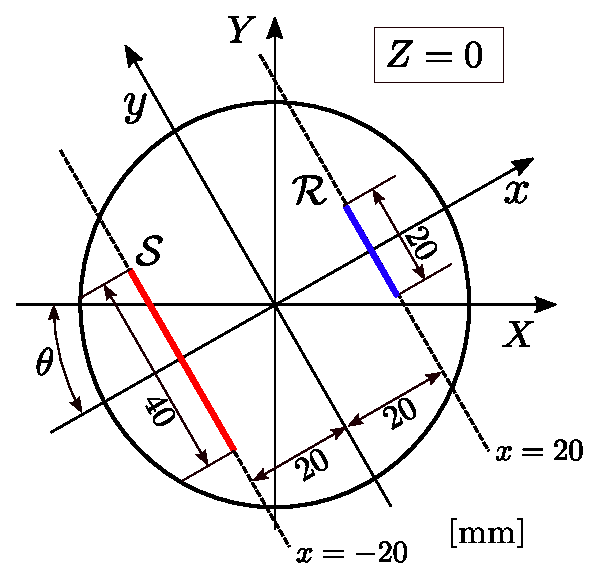
\includegraphics[width=0.5\linewidth]{Figs/fig4.eps} 
	\end{center}
	\caption{
		花崗岩コア供試体の上面における超音波送受信位置の配置.
		${\cal S}$は,ラインフォーカス探触子のカップリング位置を,
		${\cal R}$は,レーザー振動計による計測の測線を表す.
	} 
	\label{fig:fig4}
\end{figure}
%--------------------
%--------------------
\begin{figure}[h]
	\begin{center}
	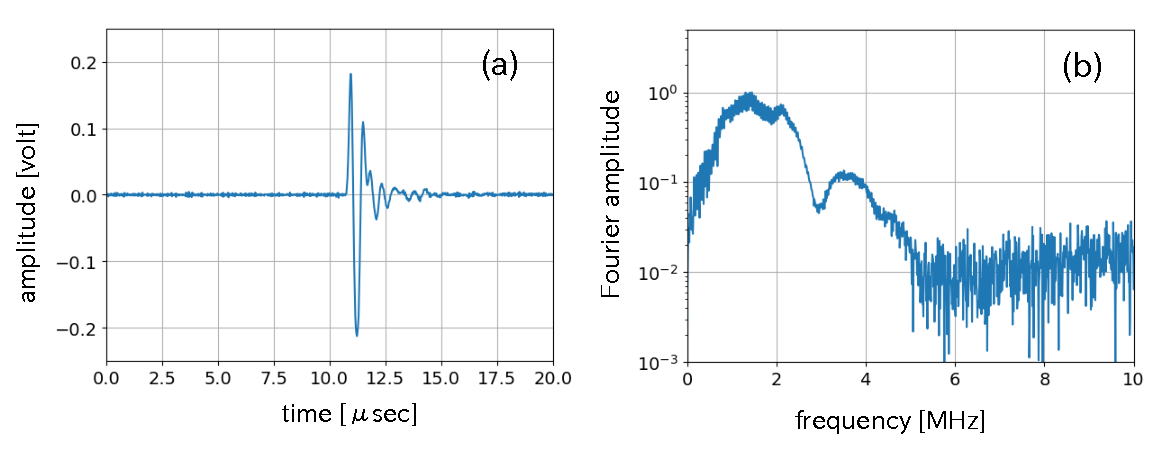
\includegraphics[width=0.9\linewidth]{Figs/fig5.eps} 
	\end{center}
	\caption{
		レーザードップラー振動計で計測した,ラインフォーカス探触子シュー先端部の振動速度波形.
	} 
	\label{fig:fig5}
\end{figure}
%--------------------
